\section{Implementierung}\label{kapitel6}
%Code erklären, Cooler Shit, Jackson, Token, Spring Sec, srtm download?, Validierung, Logger
\subsection{Webserver}
\subsubsection{Controller}
Spring MVC ermöglicht das verteilen der Anfragen an sogenannte Controller.

Diese stellen im MVC-Muster die Schicht zwischen dem Modell, sprich den Daten, und dem View, also der Ausgabe der Informationen dar.

Die Klasse des Controllers muss mit @Controller oder @RestController annotiert sein.

Über den Controller lassen sich Anfragetyp und URL u.A. anhand der Annotation ``@RequestMapping'' angeben. Ansonsten ist dies mit Spring MVC stattdessen auch mittels XML möglich.

Zusätzlich können unterschiedliche HTTP-Statuscodes zurückgegeben werden. Diese werden mit der Klasse ResponseEntity umgesetzt.

Die Annotation @RequestBody bedeutet dass es sich bei dem Parameter um den Inhalt des Anfragekörpers handelt. Dieser wird mithilfe von Jackson deserialisiert. Mehr darüber befindet sich im Abschnitt~\ref{jackson}.

Als Beispiel dient hier die Methode POST auf die URL /group, also zum Anlegen einer Gruppe:
\lstset{language=java}
\begin{lstlisting}[frame=htrbl, caption={Controller zum Erstellen einer Gruppe}, breaklines=true]
@RequestMapping(value = "group", method = RequestMethod.POST)
    public ResponseEntity<GroupDAO> create(@RequestBody @Valid CreateGroupRequest request) {
        try {
            return new ResponseEntity<GroupDAO>(Groups.createGroup(request), HttpStatus.CREATED);
        } catch(UserNotFoundException e) {
            return new ResponseEntity<GroupDAO>(HttpStatus.BAD_REQUEST);
        } catch (Exception e) {
            logger.error(e);
            return new ResponseEntity<>(HttpStatus.INTERNAL_SERVER_ERROR);
        }
   }
\end{lstlisting}
\subsubsection{Sicherheit}\label{sicherheit}
Der Webserver ist mit dem Framework Spring Security abgesichert. Die Authentifizierung war dabei kein Hauptaugenmerk der Arbeit, jedoch ist sie in Grundzügen umgesetzt worden. 

So ist der Server nur allgemein abgesichert. Hat der Nutzer ein gültiges Token hat er kompletten Zugriff auf die REST-API. Das ist natürlich keine Option für ein produktives System, das seine Nutzerdaten stärker absichern muss.

Der folgende Code befindet sich in der ApplicationContext.xml und sorgt dafür, dass sämtliche Anfragen bis auf die zum Anmelden und Registrieren von Nutzern authentifiziert sein müssen.
\lstset{language=xml}
\begin{lstlisting}[frame=htrbl, caption={AuthenticationProcessingFilter}, breaklines=true]
<security:http realm="Protected API" use-expressions="true" auto-config="false" create-session="stateless" entry-point-ref="CustomAuthenticationEntryPoint" authentication-manager-ref="authenticationManager">
        <security:custom-filter ref="authenticationTokenProcessingFilter" position="FORM_LOGIN_FILTER" />
        <security:intercept-url pattern="/login" access="permitAll"/>
        <security:intercept-url pattern="/user" method="POST" access="permitAll"/>
        <security:intercept-url pattern="/**" access="isAuthenticated()" />
</security:http>
\end{lstlisting}
\paragraph{Anmeldung}
Um sich zu anzumelden schickt der Nutzer eine Anfrage an den Server, die eine JSON mit den Attributen ``name'' und ``password'' an den Server. Stimmen diese mit den auf einem Nutzer auf der Datenbank überein antwortet der Server mit einem Token, welches der Nutzer für drei Tage nutzen kann um die authentifizierten Bereiche der API benutzen zu können. 
\begin{figure}[htb]
\centering
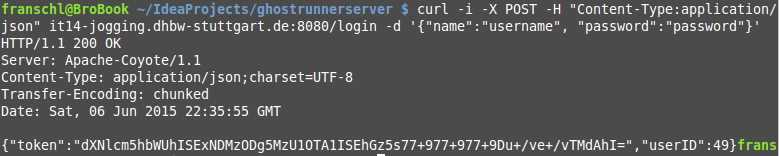
\includegraphics[width=\textwidth]{abb/curl_login}
\caption[Anmeldung]{Eine erfolgreiche Anmeldung mithilfe des Kommandozeilentools CURL}
\label{fig:Anmeldung}
\end{figure}
\paragraph{Authentifizierungstoken}
Das Authentifizierungstoken besteht, base64-dekodiert aus drei Teilen, getrennt durch jeweils drei Ausrufezeichen:
\begin{itemize}
\item Nutzername
\item Ablaufdatum des Tokens als UNIX-Zeitstempel (in Millisekunden)
\item geheimer Hash, der sich aus MD5-Hash des Nutzernamen, Salts und des Tokenablaufdatums zusammensetzt.
\end{itemize}

Dekodiert man z.B.  das erhaltene Token aus Abbildung~\ref{fig:Anmeldung} erhält man den folgenden String:
\begin{lstlisting}
username!!!1433889355905!!<eine Kette aus Sonderzeichen>
\end{lstlisting}
\paragraph{Nutzung des Sicherheitstokens}
Um sich mit dem Authentifizierungstoken am Server zu authentifizieren muss dieses bei jeder Anfrage des Klienten an den Server mitgeschickt werden.

Besonders zu Testzwecken empfiehlt es sich das Token per GET-Parameter in der URL mitzugeben. 

Eine Anfrage sieht dann z.B. so aus:
\begin{lstlisting}
it14-jogging.dhbw-stuttgart.de:8080/user/?token=<BeispielToken>
\end{lstlisting}

Eine weitere Option ist das Angeben des Tokens in der Kopzeile der Anfrage als das Attribut  ``authentication-token''.
\subsubsection{JSON - Serialisierung und Deserialisierung}\label{jackson}
Das Format der meisten Nachrichten zwischen Client und Server ist JSON.

Um den Aufwand zu minimieren und die Codeübersichtlichkeit zu maximieren wird dazu serverseitig das Tool Jackson in der Version 2.5.0 verwendet.

Es ist selbstständig in der Lage Klassen zu JSON-Objekten und Listen zu JSON-Arrays zu serialisieren und umgekehrt zu deserialisieren.

Die Einbindung erfolgt über Mavens pom.xml:
\lstset{language=xml}
\begin{lstlisting}[frame=htrbl, caption={Jacksons Abhängigkeiten in Maven}, breaklines=true]
<dependency>
	<groupId>com.fasterxml.jackson.core</groupId>
	<artifactId>jackson-core</artifactId>
	<version>2.5.0</version>
</dependency>

<dependency>
	<groupId>com.fasterxml.jackson.core</groupId>
	<artifactId>jackson-databind</artifactId>
	<version>2.5.0</version>
</dependency>

<dependency>
	<groupId>com.fasterxml.jackson.core</groupId>
	<artifactId>jackson-annotations</artifactId>
	<version>2.5.0</version>
</dependency>
\end{lstlisting}

In der mvc-dispatcher-servlet.xml wird die Bean eingebunden:
\lstset{language=xml}
\begin{lstlisting}[frame=htrbl, caption={Konfiguration von Jackson}, breaklines=true]
<bean id="jsonMessageConverter" class="org.springframework.http.converter.json.MappingJackson2HttpMessageConverter">
</bean>
\end{lstlisting}

Da Spring dank der ``component-scan''-Funktionalität von Spring MVC so konfiguriert ist, die Verzeichnisse automatisch nach Beans zu durchsuchen und diese einzubinden ist an dieser Stelle keine weitere Arbeit mehr nötig und Jackson tut seine Arbeit.

Wegen Hibernate kam es jedoch zu teils größeren Problemen mit Jackson. Diese liesen sich mittels einer weiteren Maven-Abhängigkeit eines speziell an Hibernate angepassten Jackson-Plugins und geringfügiger Änderungen im mvc-dispatcher-servlet.xml jedoch lösen:
\lstset{language=xml}
\begin{lstlisting}[frame=htrbl, caption={Einbindung von Jackson-datatype-hibernate4 in Maven}, breaklines=true]
<dependency>
	<groupId>com.fasterxml.jackson.datatype</groupId>
	<artifactId>jackson-datatype-hibernate4</artifactId>
	<version>2.4.0</version>
</dependency>
\end{lstlisting}
\lstset{language=xml}
\begin{lstlisting}[frame=htrbl, caption={Konfiguration von Jackson und Hibernate}, breaklines=true]
<mvc:annotation-driven>
        <mvc:message-converters>
            <bean class="org.springframework.http.converter.json.MappingJackson2HttpMessageConverter">
                <property name="objectMapper">
                    <bean class="com.springapp.HibernateAwareObjectMapper"/>
                </property>
            </bean>
        </mvc:message-converters>
    </mvc:annotation-driven>
\end{lstlisting}
\subsection{Android App}
\subsubsection{Höhenberechnung}
Ziel des Höhenservice der App ist es, bei übergebenem Standort in Form von Längen- und Breitengrad eine der Position entsprechenden Höhe zurückzugeben.
\paragraph{Performance}
Durch die eigenständige Implementierung des Service haben wir den Vorteil, nicht mehr von Wartezeiten der Netzwerkkommunikation abhängig zu sein. Um diesen Vorteil ausnutzen zu können, ist es nötig, den Höhenservice möglichst performant zu gestalten. Das herunterladen und parsen der vergleichsweise großen Arcascii Dateien nimmt bei dem Prozess die meiste Zeit in anspruch, sollte also während des Laufs vermieden werden. Wir haben uns entschieden, alle Dateien vor Beginn des Laufs herunterzuladen, zu parsen und alle im Umkreis des Startstandorts des Nutzers liegenden Höhendaten in einem zweidimensionalen Array im Hauptspeicher zu sichern. Auf dieses kann während dem Lauf sehr schnell zugegriffen werden.

Zusätzlich ist es wichtig, die Dateirößen zu beschränken. Statt 5x5 Grad der original SRTM Files haben wir diese in kleiner Dateien der Größe 1x1 Grad aufgeteilt. Dies entspricht immer noch einem sehr großen Bereich von 110x110 Kilometern, die Dateigröße sinkt dadurch aber auf wenige Megabyte, was für einen einmaligen Download akzeptabel ist.
\paragraph{Parsen}
Nach Download der Dateien, die der Position des Nutzers entsprechen, müssen diese geparst werden. Zunächst muss hierbei die richtige Zeile für den entsprechenden Breitengrad gefunden werden. Vereinfacht zeigt das das folgende codesnippet:
\lstset{language=java}
\begin{lstlisting}[frame=htrbl, caption={Finden der ersten benötigten Zeile}, breaklines=true]
while(row < header + latitude - elevationArray.length) \{
	srtm.readLine();
\}
\end{lstlisting}
Sobald der Startpunkt gefunden wird, werden die Zeilen in Arrays umgewandelt, und die benötigten Teilbereiche um den Nutzer in unser zweidimensionales Höhenarray gespeichert.
\lstset{language=java}
\begin{lstlisting}[frame=htrbl, caption={Füllen des Höhenarrays}, breaklines=true]
for(int i = 0; i < elevationArray.length; i++ \{
	String[] line = srtm.readLine().split(" ");
	for (int j = 0; j < arrayLength; j++) \{
                elevationArray[i][j] = Integer.parseInt(line[longitude + j]);
	\}
\}
\end{lstlisting}
Nicht beachtet wurde bei diesen Beispielen, dass Längen- und Breitengrad nicht direkt verwendet werden können, sondern zunächst in die entsprechenden Zeilen, bzw. Spalten der SRTM-Dateien umgerechnet werden müssen. Dieser Schritt hätte die Verständlichkeit des Beispielcodes unnötig erschwert.

Eine Herausforderung ergibt sich dann, wenn die Position des Nutzers sich in der Nähe von Dateigrenzen befindet. Dann ist es unter umständen nötig, bis zu vier umliegende Dateien herunterzuladen, und das Array mit Teilen aller Dateien zu initialisieren.

Ist das Array initialisiert, kann ohne weiteres langwieriges Parsen direkt auf alle Höhendaten zugegriffen werden, die während des Laufs benötigt werden.
\subsubsection{Laufberechnung}
\paragraph{Ablauf}
Wird ein Lauf gestartet, starten wir dafür einen sogenannten \textit{Service}. Dieser erlaubt es, auf Android arbeiten im Hintergrund auszuführen, und deren Ergebnisse mit der Benutzeroberfläche zu kommunizieren. Die Höhenbestimmung ist ebenfalls ein Service, der dem Laufservice bereitsteht.

Zu Beginn des Laufs wird zunächst das oben beschriebene Höhenarray initialisiert, ist dies geschehen, und kann eine Position gefunden werden, kann der Nutzer den Lauf starten. Der Android \textit{FusedLocationService} erlaubt es, regelmäßige Positionsupdates anzufordern. Für jedes Update werden folgende Schritte durchlaufen:
\begin{itemize}
\item Position mit Längen- und Breitengrad ermitteln
\item Höhe ermitteln
\item Position im GPX tracken
\item Strecke seit letztem Update berechnen
\item Steigungsmultiplikator berechnen und Streckenabschnitt multiplizieren
\item Vergangene Zeit berechnen
\item Fortschritt in Prozent berechnen
\item Falls notwendig, Fortschritt der Geister in Prozent anhand der vergangenen Zeit berechnen
\item Position berechnen
\item Überprüfen, ob die Zielstrecke erreicht wurde und gegebenenfalls Lauf hochladen und beenden
\item Benutzeroberfläche aktualisieren
\end{itemize}
\paragraph{Steigungsausgleich}
Für den Steigungsausgleich wurde eine Methode  \textit{calcDistanceModifierFromSlope(Location[] locations)} erstellt, die einen Multiplikator als Fließkommazahl zurückgibt. Das Array \textit{locations[]} beinhaltet dabei die letzten zehn Positionen.

Die Implementierung der Methode sollte möglichst flexibel sein und gleichzeitig modular in den Lauf einfügbar sein, denn es kann erst durch ausgiebiges Testen herausgefunden wie der Multiplikator wirklich berechnet werden muss. Deshalb findet die komplette Funktionalität des Höhenausgleichs an einer einzigen Stelle statt. Ein Rückgabewert von 1 entspricht keiner Streckenmodifikation, weshalb die App auch schon ohne vollständige Implementierung der Methode funktioniert.

Die primitivste Implementierung der Methode stellt ein einfaches, direktes Mapping der Steigung zwischen den letzten beiden Positionen dar. Es ist unwahrscheinlich, dass diese einen fairen Ausgleich darstellt, ist aber für anfängliche Tests gut geeignet.
\lstset{language=java}
\begin{lstlisting}[frame=htrbl, caption={Primitive Implementierung der Methode}, breaklines=true]
private double calcDistanceModifierFromSlope(Location[] locations) {
	double altitudeDelta = locations.getCurrentLocation().getAltitude() - locations.getLastLocation().getAltitude();
	double distance = locations.getLastLocation().distanceTo(locations.getCurrentLocation());
	double slope = altitudeDelta / distance;
	return slope;
}
\end{lstlisting}

Diese Methode kann optimiert werden, indem statt der Steigung ein modifizierter Wert zurückgegeben werden. Die Funktion muss nichteinmal linear sein.

Außerdem können mehr als die letzten beiden Positionen zur Berechnung herangezogen werden. So kann der Multiplikatorbonus zusätzlich erhöht werden, wenn ein steiler Streckenabschnitt über längere Zeit gelaufen wird.
